\section{Performance} \label{sec:perform}

The Start Counter was installed in Hall-D just prior to the Fall 2014 \gx{} commissioning run.  It was not until the Spring 2015 commissioning run that enough statistics were obtained with an $\mathrm{LH_{2}}$ target to perform reliable calibrations.  With the aforementioned data set, the procedures to calibrate the detector and measure it's performance were developed and deployed.

As was discussed in previous sections, the geometry of the ST nose section results in an increase of the light output as the scintillation source moves towards the downstream end.  While investigating FADC250 data under nominal beam conditions, this phenomenon was immediately observed through the pulse amplitude and pulse integral data. Figure~\ref{fig:pippvszint} illustrates that similar to the bench measurements the light output increases exponentially as the scintillation source moves towards the downstream end.
% WB one spectrum would probly be enought Amplitude or Pulse integral (here both look the same)
% EP They are in-fact the same.  They are place holders at the moment.  It will be a game-time decision as to whether or not we include both.
	\begin{figure*}[!htb]
		\centering
		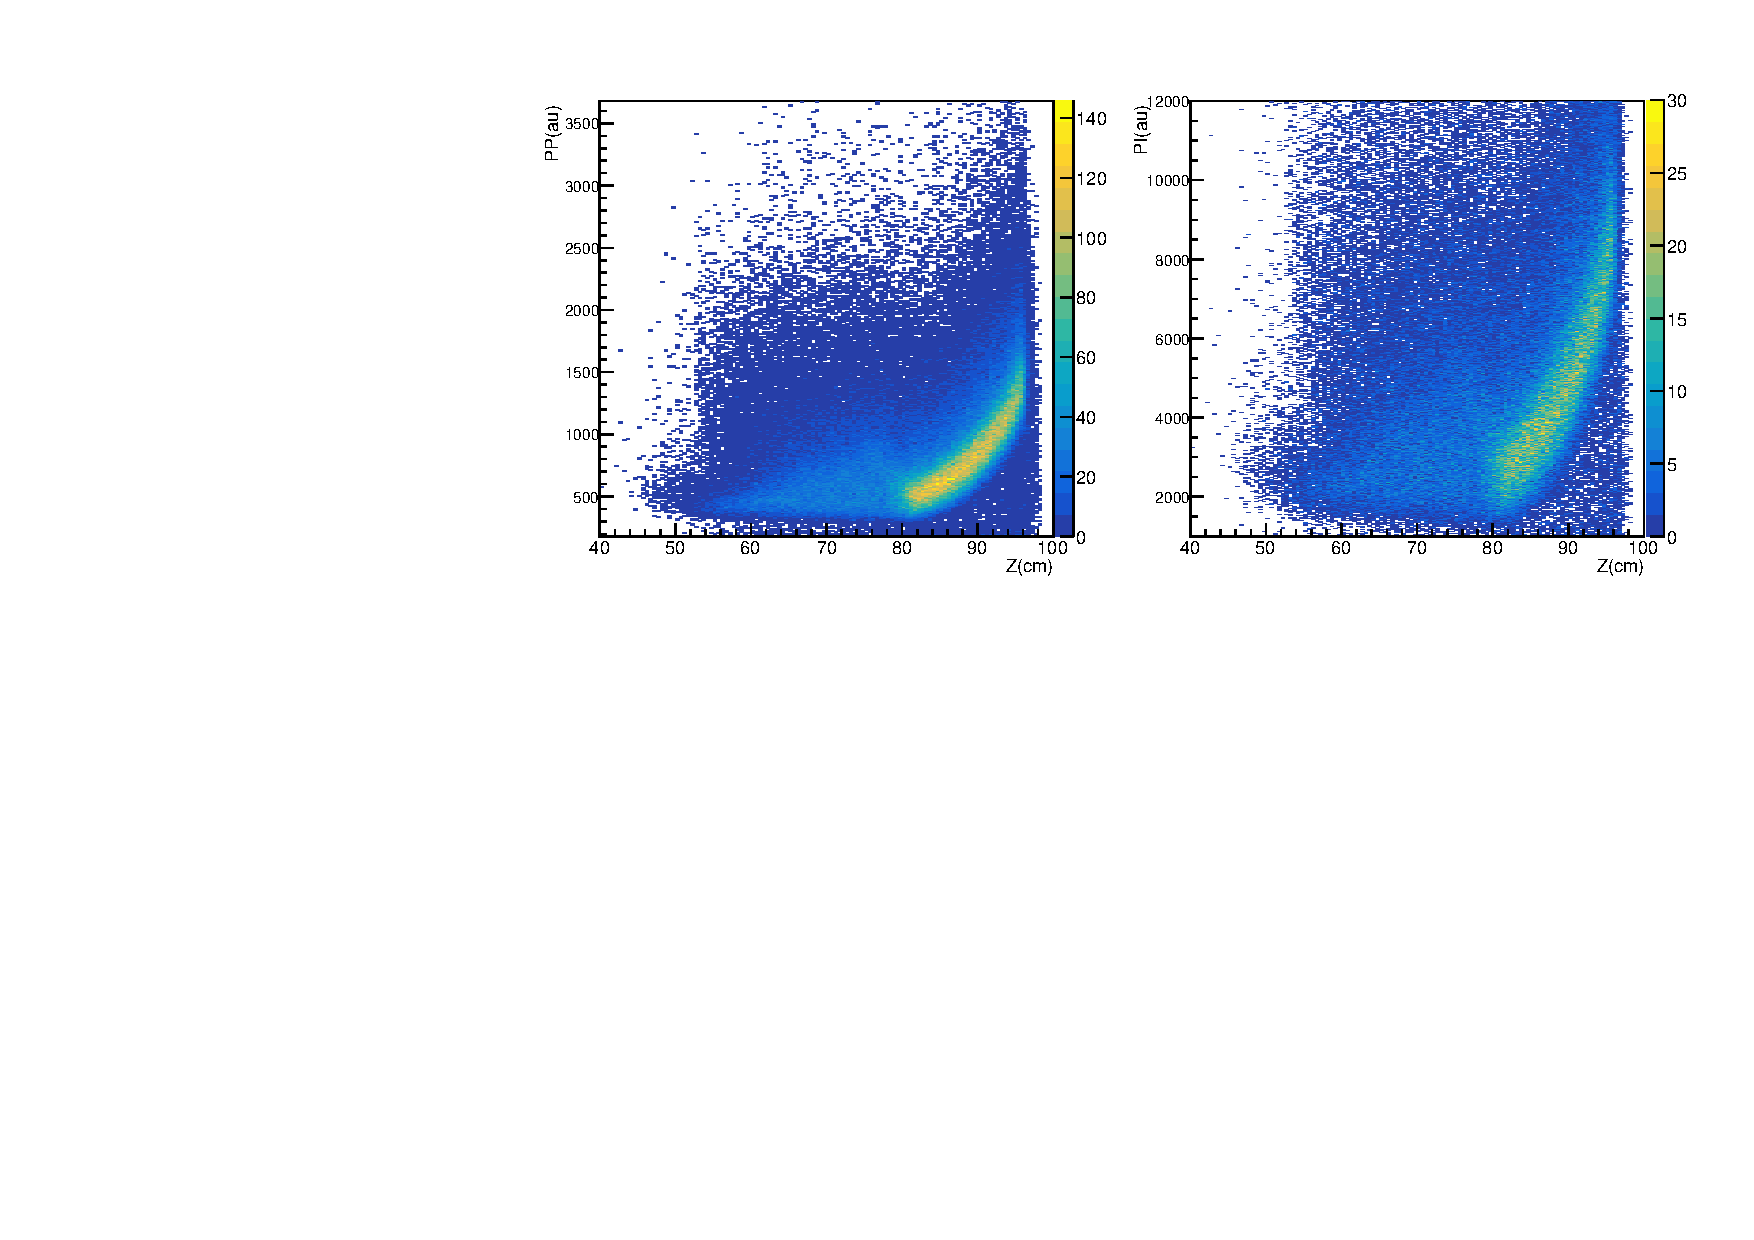
\includegraphics[width=1.0\textwidth]{performance/figs/pp_z}
		\caption{FADC spectra from the Spring 2017 run. Left: pulse amplitude versus the z-intersection of charged tracks matched to the ST. Right: pulse integral versus the z-intersection of charged tracks matched to the ST. The straight section corresponds to $40\ \mathrm{cm} < z < 80\ \mathrm{cm}$, the bend section $80\ \mathrm{cm} < z < 84\ \mathrm{cm}$, and the nose section $84\ \mathrm{cm} < z < 98\ \mathrm{cm}$.}
		\label{fig:pippvszint}
	\end{figure*}
This feature of the ST geometry is quite advantageous since the majority of the charged tracks produced under the nominal \gx{} beam conditions intersect the ST in the nose region and therefore have the largest light amount of light collected by the SiPM's as the upstream end.

%Once the proper attenuation corrections were applied to the data, the PID capabilities of the ST were greatly enhanced.  Figure ~\ref{fig:dEdx_vs_p_uncorr}-b illustrates the PID capability of charged tracks intersecting the ST.  As compared to Fig.~\ref{fig:dEdx_vs_p_uncorr}-a, the reliable separation of protons and other hadrons occurs for charged tracks with $p < 1.1\ GeV/c$ which is a factor two improvement from the uncalibrated data.
%	\begin{figure}[!htb]
%		\centering
%		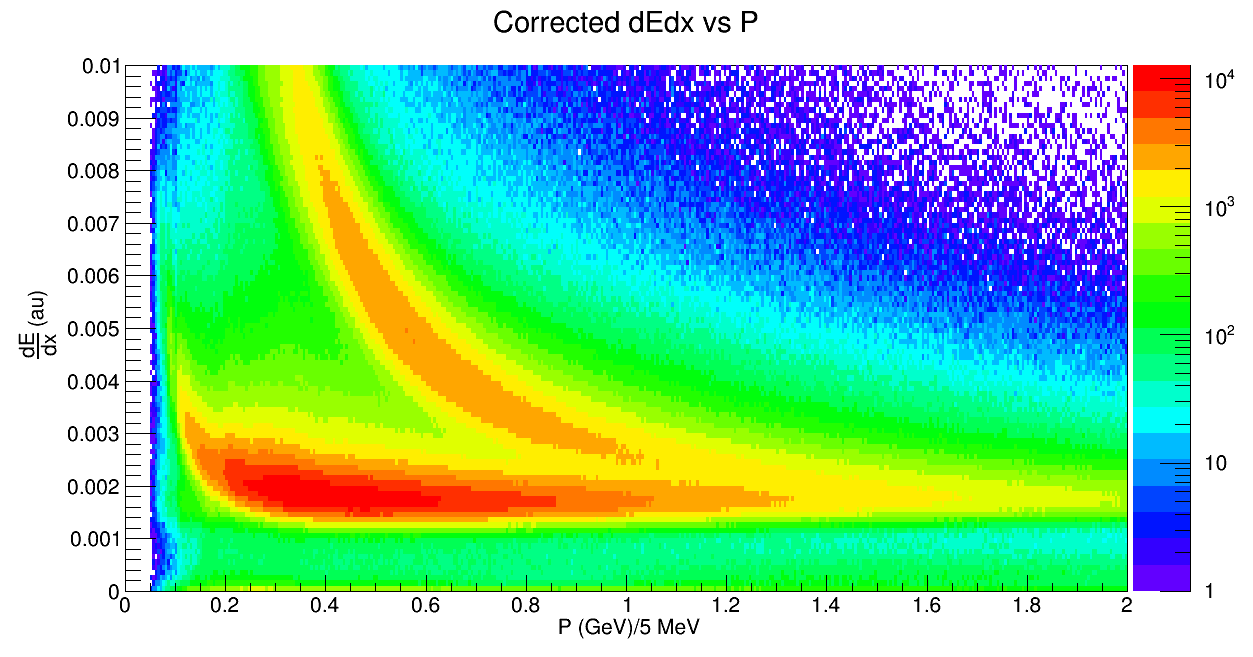
\includegraphics[width=1.0\columnwidth]{performance/figs/dEdx_vs_p_corr}
%		\caption{Typical corrected $dE/dx\ vs.\ p$ distribution in the Start Counter.  Shown is the corrected $dE/dx\ vs.\ p$ distribution for tracks matched to the Start Counter in the Spring 2017 run. The ``banana band'' corresponds to protons while the horizontal band corresponds to charged electrons, pions, and kaons.  It is clear that pion/proton separation is achievable for tracks with $p < 1.1\ GeV/c$.}
%		\label{fig:dEdx_vs_p_corr}
%	\end{figure}  

After the previously discussed time-walk and propagation time corrections were complete, it was then possible to utilize the ST to measure the time of charged track vertices for tracks that are matched to the ST.  The vertex time is defined to be the time in which a polarized Bremsstrahlung photon interacted with the $\mathrm{LH_{2}}$ target and produced a charged track that intersected the ST.  An identical charged track selection process as outlined in Sec.~\ref{sec:calib_ptc} was utilized so that the time resolution of tracks matched to the ST could be measured.

The equation to calculate the ST measure of the vertex time is given by Eq.~\ref{eq:st_prop_time}.  
%In an identical manner outlined in Sec.~\ref{sec:calib_ptc}, $T^{RF}_{vertex}$ must be ``stepped'' to the time the charged track vertex was produced so as to obtain a proper measure of the RF time.  
The resulting distribution in the time difference of these times provides a measure of the ST time resolution and is seen in Fig. \ref{fig:beam_tof_corr_chan_15}.
	\begin{figure}[!htb]
		\centering
		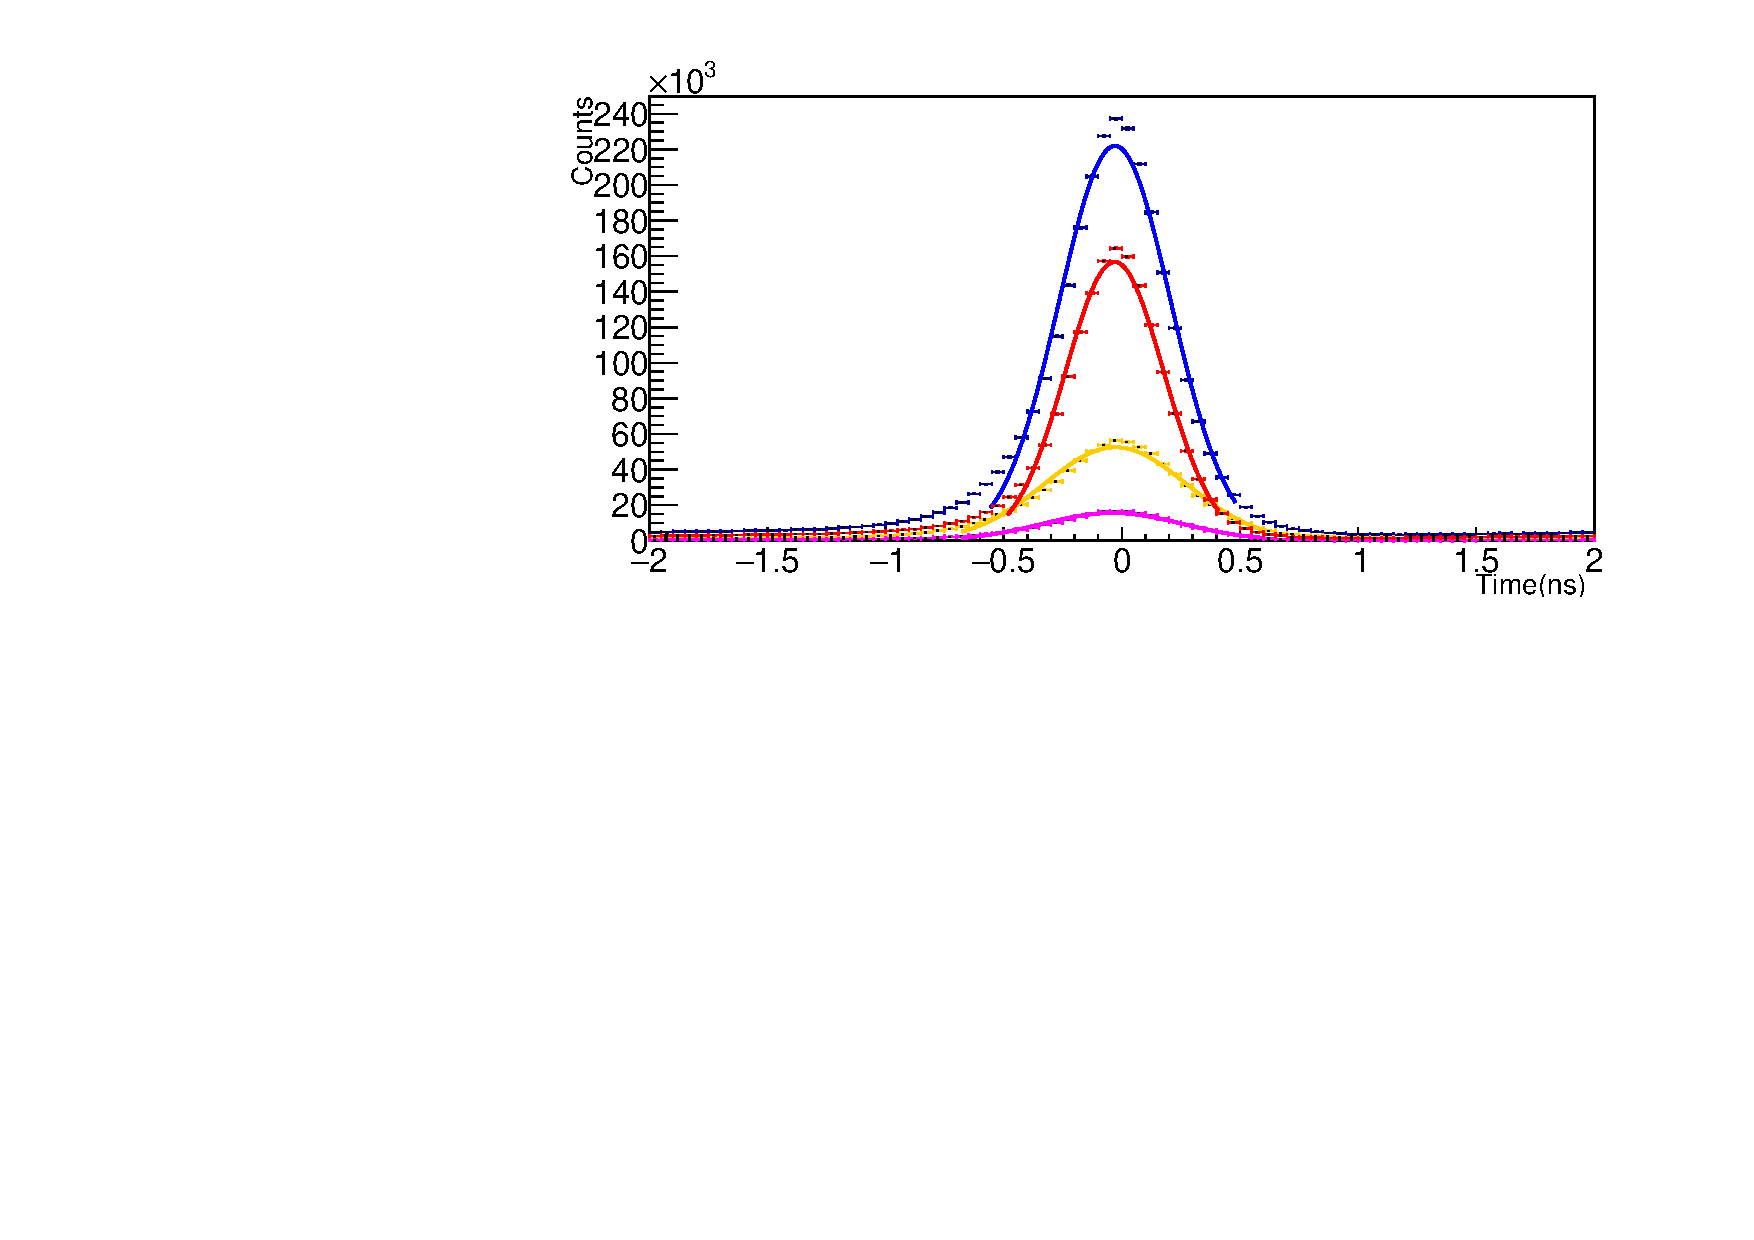
\includegraphics[width=1.08\linewidth]{performance/figs/TR_15}
		\caption[Typical Start Counter/RF time resolution distribution]{Typical Start Counter/RF time resolution distribution.  Shown is the time resolution distribution for sector 15 during the Spring 2017 run 30279. The x-axis is the time difference between $T^{ST}_{vertex}$ and $T^{BB}_{vertex}$. The orange histogram is the resolution in the straight section. The magenta and red histograms correspond to the resolution in the bend and nose sections respectively. The blue histogram is a sum of the three sections and corresponds to the resolution along the entire length of the paddle.}
		\label{fig:beam_tof_corr_chan_15}
	\end{figure}
	
\begin{figure}[!htb]
		\centering
		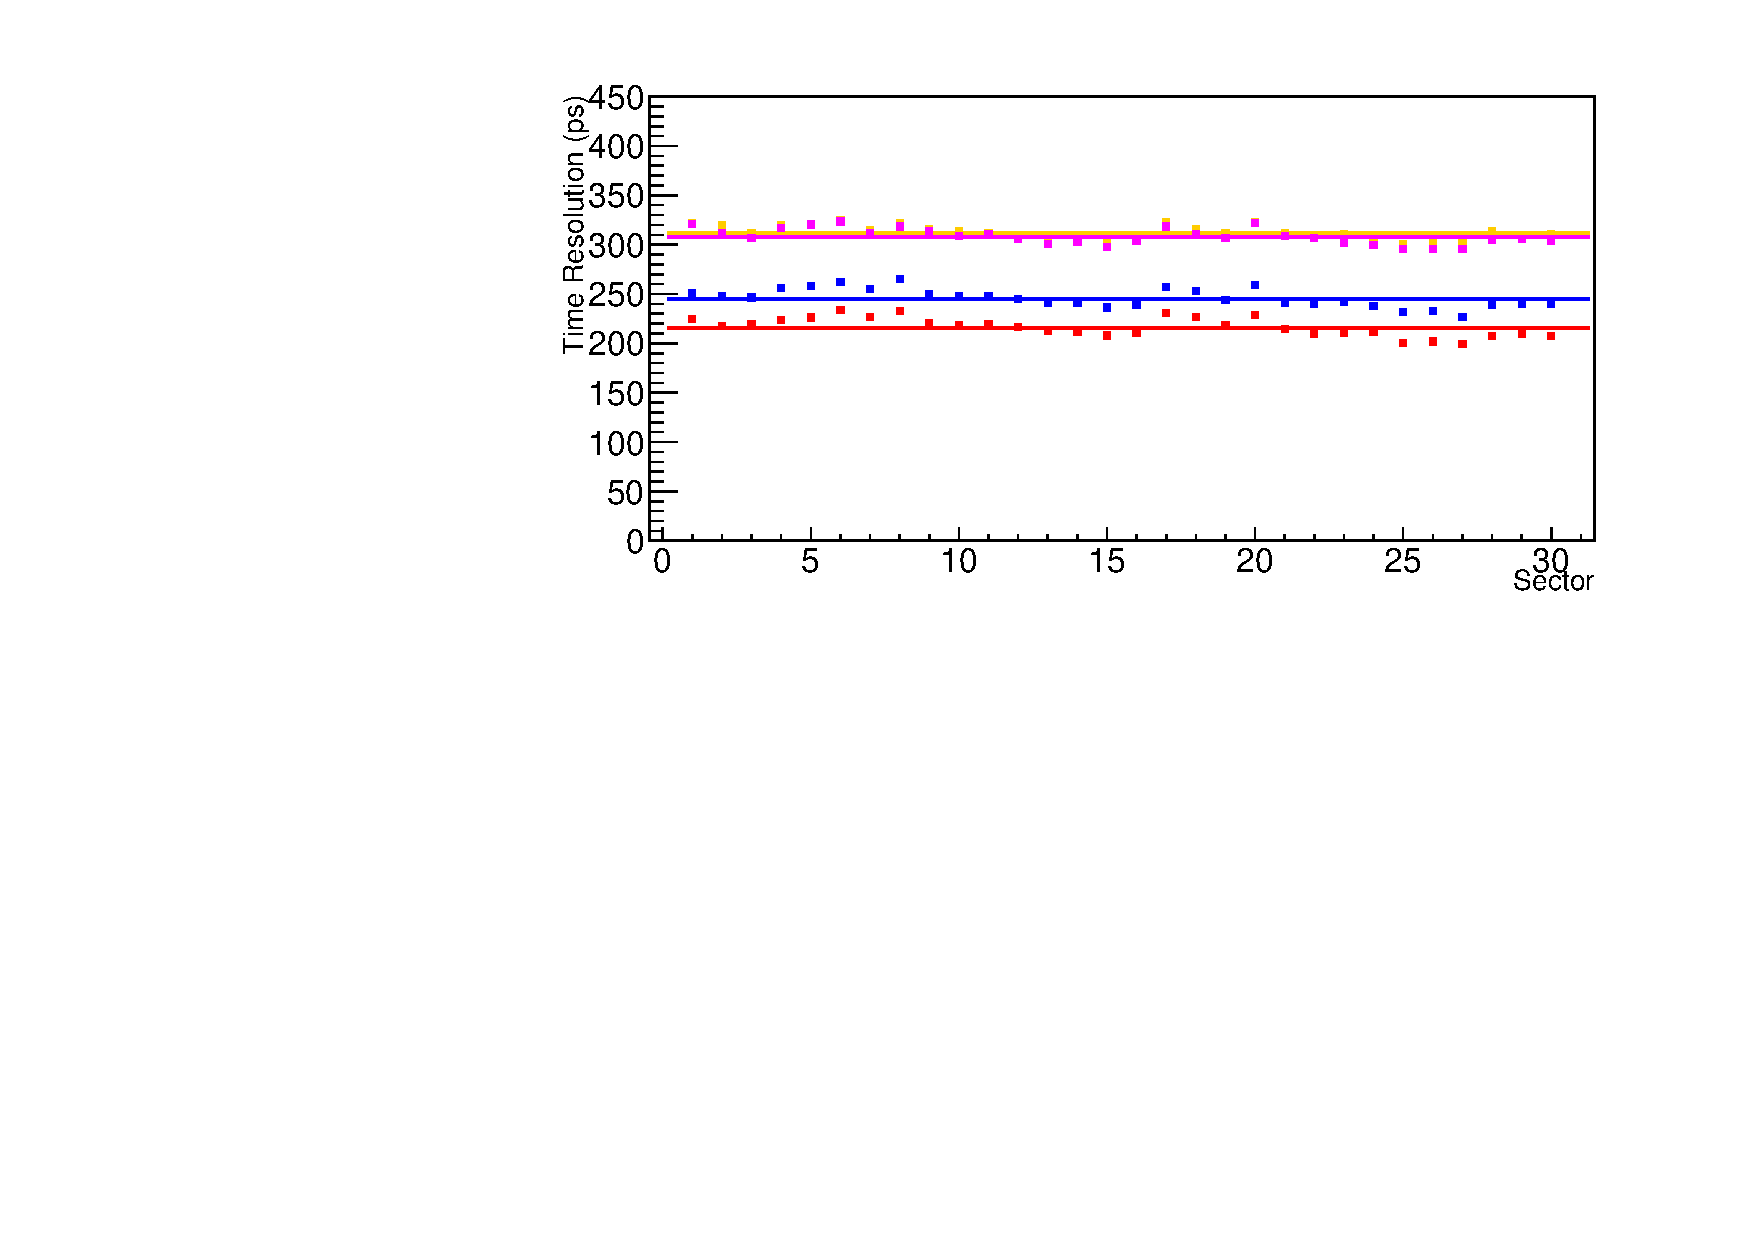
\includegraphics[width=1.08\columnwidth]{performance/figs/TR_All}
		\caption{ST time resolutions as a function of sector number (Blue line). Orange and magenta lines are the average time resolution for the straight and bend sections respectively. The nose section resolution is greatly enhanced due to the exponential increase in light output (red).}
		\label{fig:timeresallinset}
	\end{figure}		
The aforementioned fits were then carried out for each of the ST sectors with $\sigma$, and its associated error being calculated.  Then a weighted average of the 30 $\sigma$'s were calculated so that the ST could have its time resolution characterized in its entirety.  The same procedure was also conducted for the three individual sections.  Figure \ref{fig:timeresallinset} illustrates the uniformity in time resolution among all sectors of the ST. It indicates also that the average time resolution of 245~ps is well below the design resolution of 350~ps.
\begin{table}[h]
	\centering
	\begin{tabular}{|c|c|c|c|c|}
		\hline  \textbf{Section} & $\mathbf{\sigma_{all}}$ & $\mathbf{\sigma_{straight}}$ & $\mathbf{\sigma_{bend}}$ & $\mathbf{\sigma_{nose}}$ \\ 
		\hline $\mathbf{\sigma_{avg}}$ & 245 ps & 314 ps & 309 ps & 216 ps \\ 
		\hline 
	\end{tabular}
	\caption[Average time resolutions by section]{Average time resolutions by section. Shown is the average of all 30 ST sectors by independent geometrical regions.}
	\label{tab:time_res_section}
\end{table}

Table \ref{tab:time_res_section} details the weighted average time resolution of all the ST sectors in the different geometrical regions.

It is clear from Table \ref{tab:time_res_section} that what is observed is that measurements made with beam data exhibit the same phenomenon of substantial improvement in light collection, and thus time resolution, as light is produced further downstream in the nose region.

When these time resolution measurements were conducted with data collected in Spring 2017, approximately 3 years had elapsed since the paddles were first tested on the bench at FIU.  Prior experience with degrading scintillators indicates that degradation in time resolution will be visible in a matter of weeks.  However, after 3 years no degradation has been observed and the ST is still performing well below design resolution.